\chapter{Điều khiển truy cập trên dữ liệu mã hóa}

\section{Tổng quan về kiểm soát truy cập trên cơ sở dữ liệu}

Kiểm soát truy cập là vấn đề quan trọng trong bất kỳ cơ quan, tổ chức hay hệ
thống nào. Từ thời cổ đại, con người đã phát minh ra các phương pháp kiểm soát truy
cập khác nhau: sử dụng lệnh bài, giấy tờ hợp lệ… để ra vào các khu vực giới hạn. Trong
lĩnh vực công nghệ thông tin hiện đại, kiểm soát truy cập là khả năng của hệ thống để
xác định xem người dùng có thể truy cập vào một phần dữ liệu cụ thể được lưu giữ trong
hệ thống máy tính và môi trường hoạt động liên quan của nó hay không \cite{emms1987definition}. Nó bao gồm
hai thành phần chính là xác thực \textit{(authentication)} và ủy quyền \textit{(authorization)}. Xác thực
là phương pháp xác minh danh tính của người đang truy cập cơ sở dữ liệu. Ủy quyền là
phương pháp xác định người dùng có được phép truy cập vào dữ liệu hoặc thực hiện các
thao tác trên dữ liệu đó hay không. Nếu thiếu một trong hai yếu tố này, dữ liệu không
được bảo vệ. \\
\indent Các chính sách kiểm soát truy cập có thể chia thành ba nhóm chính chính: Điều
khiển truy cập tùy ý (DAC), Điều khiển truy cập bắt buộc (MAC) và Điều khiển truy cập
theo vai trò (RBAC) \cite{sandhu1996role}.
\subsection{Điều khiển truy cập tùy ý (DAC).}
Ở mô hình điều khiển truy cập DAC, chủ sở hữu kiểm soát quyền truy cập nhưng
chỉ với bản gốc, không phải với bản sao. Mô hình gồm ba thành phần: chủ thể (subject),
quyền truy cập (access) và đối tượng (object). Trong DAC, chủ sở hữu dữ liệu quyết
định quyền truy cập của các chủ thể khác trên đối tượng do mình sở hữu, xem\ref{fig:chap2-dac}. 
\begin{figure}
    \centering
    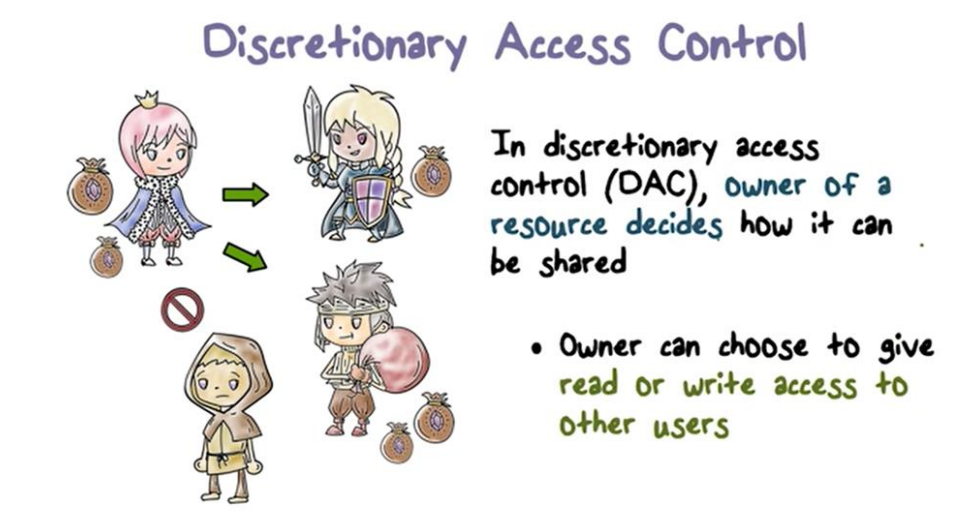
\includegraphics[scale=0.5]{graphics/chapter-2/chap2-dac.png}
    \caption{Minh họa mô hình DAC}
    \label{fig:chap2-dac}
\end{figure}
\indent Tuy nhiên, mô hình này có nhược điểm lớn là việc trao quyền kiểm soát truy cập
của đối tượng chủ sở hữu của nó có thể làm tiết lộ dữ liệu cho những người không có
quyền truy cập hợp pháp với nó. Chúng ta không thể đảm bảo rằng chủ sở hữu dữ liệu
là tuyệt đối tin tưởng được. Trong trường hợp chủ sở hữu có thể tin tưởng, khả năng chủ
sở hữu quyết định sai các quyền truy cập trên các tài nguyên của mình có thể gây nên đổ
vỡ hệ thống. Các chủ thể xấu tồn tại trong hệ thống có thể lợi dụng sự thiếu hiểu biết hoặc sai lầm của chủ sở hữu dữ liệu, kết hợp với nhau để chiếm đoạt tài nguyên bất hợp
pháp. \\
Giả sử hệ thống chúng ta có các thành phần như mô tả trong bảng sau: \\

\begin{table}[ht]
    \centering
    \caption{Ví dụ về kiểm soát truy cập DAC}
    \label{tab:chap2-dac-example}
    \begin{tabular}{| p{.25\textwidth} | p{.25\textwidth} | p{.25\textwidth} |}
        \hline
        \textbf{Chủ thể} & \textbf{Quyền truy cập} & \textbf{Đối tượng} \\
        \hline
        A & R & File F \\
        \hline
        A & W & File F \\
        \hline
        A & W & File G \\
        \hline
        B & R & File G \\
        \hline
    \end{tabular}
\end{table}
Theo như bảng trên, B không thể đọc được các nội dung trong file F do không có
quyền R trên file F. Tuy nhiên, tận dụng lỗ hổng của mô hình DAC, chủ thể A có thể
đọc các nội dung trên file F, thực hiện ghi nó vào file G. Từ đó, B có thể đọc được nội
dung của file F mà không cần có quyền gì trên file F (xem \ref{fig:chap2-troyjan-dac}). Vì những rủi ro của nó, trong các hệ thống hiện đại ngày nay, các công ty, tổ chức hạn chế và hầu như không sử dụng mô hình kiểm soát truy cập DAC. 
\begin{figure}
    \centering
    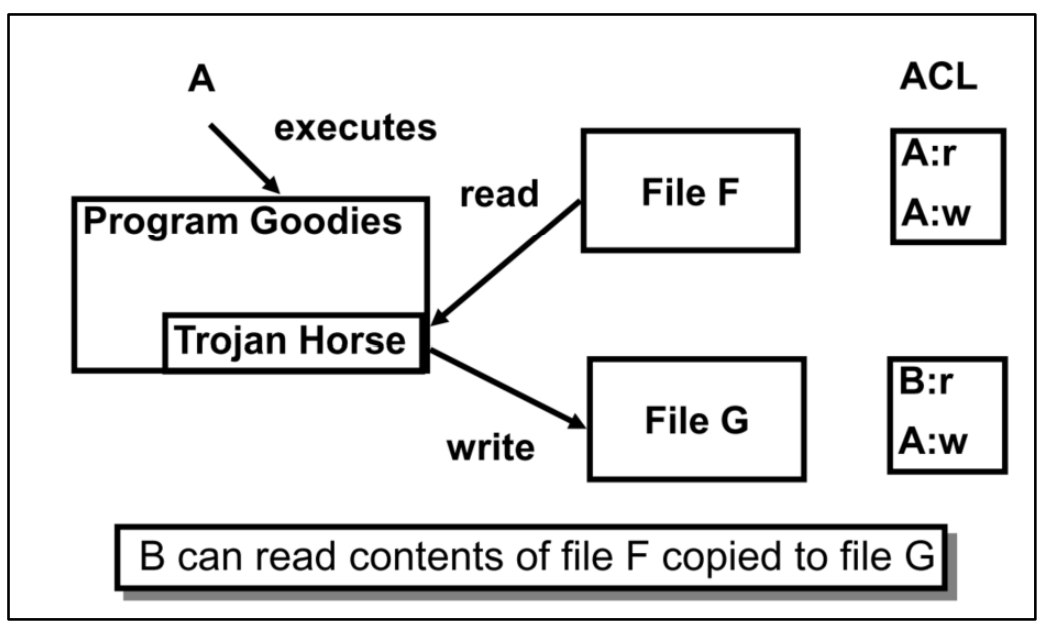
\includegraphics[scale=0.5]{graphics/chapter-2/chap2-troyjan-dac.png}
    \caption{Lỗ hổng trojan horse trong mô hình DAC \cite{sandhu1996role}}
    \label{fig:chap2-troyjan-dac}
\end{figure}
\subsection{Điều khiển truy cập bắt buộc (MAC).}

Trong mô hình MAC, quyền truy cập đối với các đối tượng không được quyết
định bởi chủ thể mà được quyết định bởi một người (hoặc hệ thống) quản trị. Các chủ
thể và đối tượng được gắn các nhãn tương ứng với mức độ “nhạy cảm” của họ và được
sắp xếp một cách có trật tự (xem ). MAC áp dụng hai quy tắc chính đó là
no read-up và no write-down. Mối quan hệ giữa các luồng thông tin trong hệ thống này
là phản xạ, bắc cầu và phản đối xứng. Điểm mạnh của MAC là đảm bảo bí mật của thông
tin và cung cấp biện pháp chống lại phương pháp tấn công trojan horse. Điều này đạt
được do các nhãn của đối tượng được truyền qua các bản sao và ngăn chặn việc hạ cấp
nhãn của đối tượng, từ đó đảm bảo dữ liệu không thể chuyển từ mức độ “nhạy cảm” cao
xuống thấp \cite{nyanchama1996modeling}. 
\begin{figure}
    \centering
    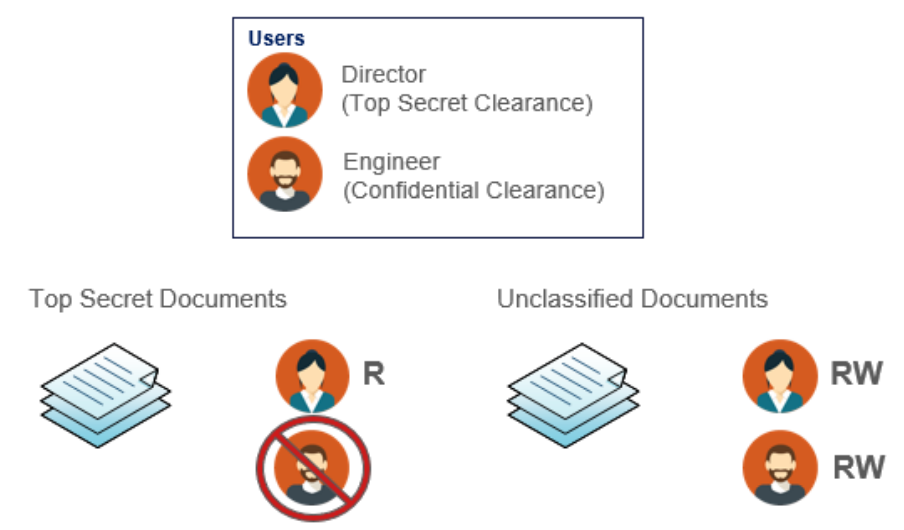
\includegraphics[scale=0.5]{graphics/chapter-2/chap2-mac.png}
    \caption{Minh họa mô hình MAC}
    \label{fig:chap2-mac}
\end{figure}
\indent Khi nhắc tới MAC, mô hình Bell-La Padula \cite{bell1973secure} thường được nhắc tới thường xuyên nhất. Nhóm tác giả phân tích rất khái quát về mô hình Bell-La Padula nhằm đại
diện cho phương pháp MAC. Trong mô hình Bell-La Padula, có một tập hợp nhãn phân loại (top-secret, secret,
confidential, unclassified) được xác định hoàn toàn. Bên cạnh đó, có một danh sách các
danh mục không được phân loại. Sự kết hợp của một nhãn và một thành phần con của
danh mục được gọi là mức bảo mật. Mức bảo mật được sắp xếp một phần và tạo thành
một mạng lưới \cite{osborn1997mandatory}. Trong mạng lưới này, các chủ thể không được đọc các tài liệu có nhãn mức bảo
mật cao hơn mình, đồng thời không được viết ra các tài liệu có nhãn bảo mật thấp hơn
mình. Nghĩa là một chủ thể có mức bảo mật secret thì không thể đọc được tài liệu có
nhãn top-secret nhưng có thể đọc được các tài liệu có nhãn bằng hoặc thấp hơn mình
(secret, confidential, unclassified). Bên cạnh đó, chủ thể này cũng không thể tạo ra các
tài liệu có nhãn bảo mật thấp hơn nhãn của mình. Phương pháp kiểm soát truy cập này rất phù hợp trong môi trường cần đề cao tính bí mật của thông tin như quân sự, ngoại
giao (xem ví dụ hình \ref{fig:chap2-blp-model}).
\begin{figure}
    \centering
    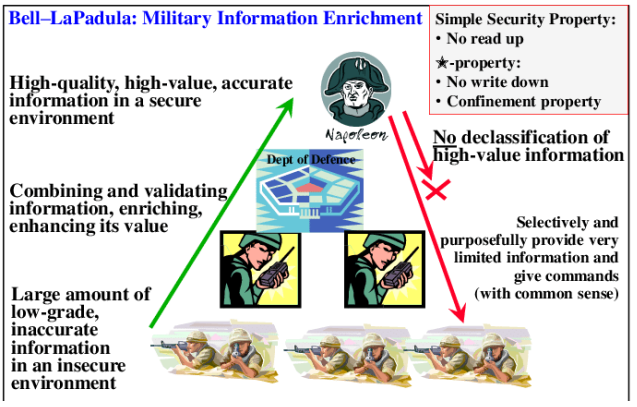
\includegraphics[scale=0.6]{graphics/chapter-2/chap2-blp-model.png}
    \caption{Ví dụ về mô hình Bell-La Padula}
    \label{fig:chap2-blp-model}
\end{figure}
Tuy nhiên, do sự đa dạng các yêu cầu, đặc biệt là mong môi trường điện toán đám
mây với lượng truy cập lớn, các quy tắc và định lý bảo mật hiện tại trong BLP không thể
thích ứng được \cite{tang2018self}.  Các hạn chế của nó dần dần bộc lộ trong quá trình phát triển lý
thuyết về bảo mật.
Giả sử, trong hệ thống ban đầu chỉ có một một loại phân cấp, khi một chủ thể yêu
cầu truy cập vào đối tượng. Trong trường hợp này, do tất cả chủ thể và đối tượng đều
được phân cấp là thấp nhất, yêu cầu này đương nhiên được chấp thuận theo BLP, nhưng
đó rõ ràng là rủi ro lớn \cite{mclean1990security}. \\
\indent Nhiều giải pháp cải thiện mô hình BLP được đưa ra để phù hợp với sự phát triển
của lý thuyết bảo mật: đề xuất một phương pháp có thể xác định các chủ thể một cách
linh động bằng cách cung cấp các phương pháp chuyển đổi trạng thái trong BLP \cite{zhu2016application}; định nghĩa các chủ thể, đối tượng và quy tắc bảo mật trong network domain, cung cấp
các quy tắc để hạn chế hành vi của hệ thống \cite{ou2009research}. 
\indent Mặc dù các nghiên cứu đã có nhiều nỗ lực để cải thiện BLP và các ứng dụng của
nó, nhưng mô hình chủ động điều chỉnh với những thay đổi ít khi được đề cập đến. Các
nghiên cứu ít chú đến các hệ thống yêu cầu thời gian thực, thiếu khả năng thay đổi theo
bối cảnh \cite{yang2019using}.
\subsection{Điều khiển truy cập theo vai trò (RBAC)}
Phương pháp điều khiển truy cập dựa theo vai trò thực hiện dựa trên chính sách
quy định quyền truy cập của người dùng vào các tài nguyên trên cơ sở mà người dùng
thực hiện. Nó yêu cầu xác định cụ thể từng vai trò trong hệ thống. Theo đó, vai trò là
một tập hợp các quyền sử dụng các tài nguyên phù hợp với chức năng và công việc của
một người, là một tập hợp các hành động và trách nhiệm liên quan đến một hoạt động
cụ thể. Thay vì chỉ định tất cả các quyền mà người dùng được phép thực thi, các quyền
truy cập được chỉ định cho các vai trò. Người dùng được thêm vào các tập hợp vai trò
mà thông qua đó, được phép thực thi các quyền của vai trò đó \cite{hu2006assessment}. 
\indent Theo thời gian, các doanh nghiệp nhận thấy nhu cầu vượt ra ngoài các định nghĩa
về nhóm người dùng và quyền của RBAC. Chúng cần bao gồm các thuộc tính linh động
như thời gian trong ngày, vị trí của người dùng. Các hệ thống phân tán và thay đổi liên
tục, kiểm soát truy cập dựa trên thuộc tính là một lựa chọn hoặc thay thế, hoặc bổ trợ
cho RBAC. ABAC sử dụng các đối tượng được gắn nhãn và thuộc tính người dùng thay
vì quyền để kiểm soát một cách linh hoạt.
\begin{figure}
    \centering
    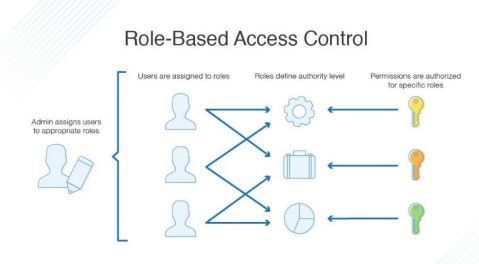
\includegraphics[scale=0.7]{graphics/chapter-2/chap2-rbac.png}
    \caption{Minh họa về RBAC}
    \label{fig:enter-label}
\end{figure}
\subsection{Điều khiển truy cập dựa theo thuộc tính (ABAC)}
ABAC là một mô hình logic điều khiển truy cập vào các đối tượng bằng cách
đánh giá các quy tắc dựa trên các thuộc tính của các đối tượng và chủ thể, các hoạt động
và môi trường liên quan đến một ngữ cảnh yêu cầu cụ thể. Nó cho phép kiểm soát truy
cập chính xác hơn bằng cách cho phép số lượng lớn đầu vào rời rạc tham gia vào quá
trình quyết định quyền truy cập, và do đó cung cấp một lượng lớn hơn các kết hợp có
thể có của các thuộc tính để phản anh một chính sách lớn hơn rất nhiều so với các phương
pháp khác. Nó chỉ bị giới hạn ngôn bởi ngôn ngữ tính toán và sự phong phú của các
thuộc tính có sẵn \cite{hu2015attribute}. 
\indent Mô hình điều khiển truy cập ABAC cơ bản có 3 bước: chủ thể yêu cầu một truy
cập (đọc, ghi, thực thi…) tới một đối tượng cụ thể; hệ thống kiểm tra và đánh giá các
thuộc tính mà chủ thể cung cấp; chủ thể được cho phép truy cập tài nguyên nếu là người
dùng xác thực và bị cấm nếu không xác thực. 
\begin{figure}
    \centering
    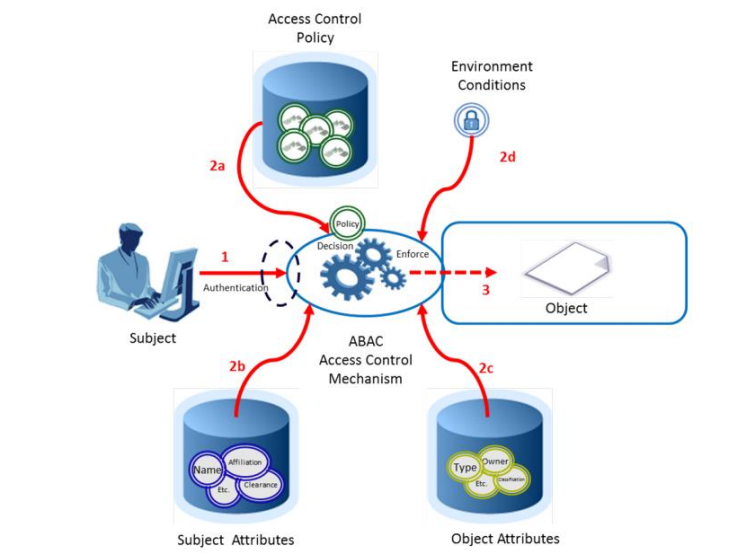
\includegraphics[scale=0.5]{graphics/chapter-2/chap2-basic-abac.png}
    \caption{Mô hình ABAC cơ bản \cite{hu2013guide}}
    \label{fig:chap2-basic-abac}
\end{figure} 
\indent ABAC cho phép đưa ra các quyết định kiểm soát truy cập mà không cần chủ thể
biết trước về đối tượng. Với phương pháp khái quát thuộc tính được xác định nhất quán
giữa các tổ chức, nó tránh được nhu cầu xác minh quyền truy cập rõ ràng của các chủ
thể với các đối tượng, nghĩa là chủ thể không biết rõ mình có quyền truy cập được đến
đối tượng hay không khi chưa có nhu cầu truy cập tài nguyên đó, trong khi đối với
RBAC, các chủ thể trong một tập vai trò biết rõ và tường minh các quyền của mình đối
với đối tượng cụ thể. ABAC cho phép sự linh hoạt trong một doanh nghiệp lớn và rất
lớn, nơi việc quản lý các danh sách vai trò và nhóm kiểm soát truy cập tốn thời gian và
phức tạp. Nếu các thuộc tính được xác định nhất quán, các thủ tục xác thực và cho phép
truy cập có thể được thực thi và quản lý trong các cơ sở khác nhau, đồng thời duy trì
mức độ bảo mật thích hợp trong tổ chức mới. Ví dụ một chủ thể có thể xác thực và truy
cập tài nguyên trong bệnh viện này và sau đó được ủy quyền để truy cập các tài nguyên
trên bệnh viện khác tương tự như đối với bệnh viện cũ, nhờ các giá trị thuộc tính được
xác định nhất quán từ trước. Sau khi hoàn thành vai trò tại cơ sở tạm thời, việc loại bỏ quyền được cấp tạm thời được thực hiện dễ dàng mà không ảnh hưởng tới những người
dùng khác trong hệ thống. 
\indent Kỹ thuật kiểm soát truy cập quản lý dựa trên từng giá trị thuộc tính do người sở
hữu dữ liệu định nghĩa. Nó hỗ trợ quản lý các nhóm người dùng có cùng chính sách truy
cập như kỹ thuật kiểm soát dựa trên vai trò, nhưng cá nhân hóa hơn nhờ áp dụng phương
pháp dẫn xuất khóa nhóm. Người quản trị không cần phải thay đổi nhóm vai trò của từng
người dùng mỗi khi họ thay đổi nhiệm vụ hoặc rời khỏi hệ thống mà việc phân bố lại
nhóm trong hệ thống được thực hiện một cách tự động hoàn toàn. Khi mỗi người dùng
có thay đổi về thuộc tính, gia nhập hoặc rời khỏi hệ thống, người quản trị chỉnh sửa
tương ứng giá trị thuộc tính của họ, những người dùng khác trong hệ thống không bị ảnh
hưởng. Thông thường, chính sách truy cập quy định một chủ thể s có thể truy cập vào
tài nguyên r trong điều kiện bảo mật \textbf{e} được biểu diễn bằng biểu thức đại số bởi 3 biến \textbf{s, r, e} như sau:
\begin{center}
$can\_access(s, r, e) \leftarrow f(ATTR_{s},ATTR_{r}, ATTR_{e})$ \cite{yuan2005attributed}
\end{center} với $ATTR_{s}$ là thuộc tính của chủ thể $s$. 
\indent Thông thường, một người dùng sẽ được chỉ định (hủy chỉ định) một cách tự động
vào các nhóm nếu họ đáp ứng các điều kiện thành viên nhóm. Một điều quan trọng khác
là cơ chế quản lý khóa nhóm, bởi mục tiêu các nhóm thường là chia sẻ dữ liệu. Do đó
dữ liệu phải được mã hóa với các khóa chỉ được cung cấp cho các thành viên của nhóm.
Việc quản lý những khóa, bao gồm các lựa chọn, phân phối, lưu trữ, cập nhật yêu cầu
phương pháp quản lý khóa nhóm dựa trên thuộc tính. Theo đó các khóa nhóm được gán
cho người dùng dựa trên các thuộc tính nhận dạng của họ. 
\indent Khi nhóm thay đổi, khóa nhóm mới phải được chia sẻ với các thành viên hiện có,
để một thành viên nhóm mới không thể truy cập dữ liệu được truyền trước khi họ tham
gia nhóm và một người dùng đã rời đi khỏi nhóm không thể truy cập dữ liệu của nhóm.
Một vấn đề khác là bảo vệ chống lại các cuộc tấn công thông đồng mà qua đó, một nhóm người dùng gian lận thông đồng có thể có được khóa nhóm bằng cách tập hợp những
khóa của nhau, sau đó lấy khóa nhóm và đáng ra họ không được phép lấy riêng lẻ. 
\indent Mặc dù ABAC có thể hỗ trợ trong việc chia sẻ thông tin doanh nghiệp, nhưng khi
triển khai trên quy mô doanh nghiệp, tập hợp các khả năng cần thiết để thực hiện trở nên
phức tạp hơn. Ở cấp độ doanh nghiệp, quy mô lớn đòi hỏi khả năng quản lý phức tạp và
đôi khi cần được thiết lập một cách độc lập. Hình \ref{fig:chap2-enterprise-abac} trình bày chi tiết các thành phần cần thiết khi triển khai ABAC trong
doanh nghiệp. Hầu hết các doanh nghiệp hiện tại đều có thể đáp ứng được các thành
phần trong sơ đồ như có hình thức quản lý và thông tin xác thực nhân viên. Tuy nhiên,
các quy tắc thường được viết thành các loại văn bản mà con người có thể đọc được và
thiết kế thành các phần mềm riêng lẻ. Để có thể triển khai ABAC trong doanh nghiệp
được hiệu quả, các chính sách quản lý phải lưu dưới dạng máy có thể đọc được. Từ đó
có thể triển khai quản lý các chủ thể và đối tượng được toàn diện.
\begin{figure}
    \centering
    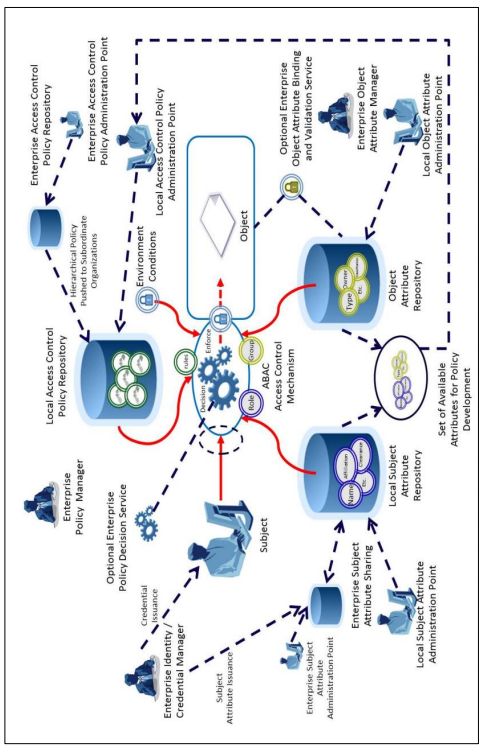
\includegraphics{graphics/chapter-2/chap2-enterprise-abac.png}
    \caption{Ví dụ về ABAC trong doanh nghiệp \cite{hu2013guide}}
    \label{fig:chap2-enterprise-abac}
\end{figure}

Trong ABAC, chúng ta không cần định nghĩa các vai trò cụ thể và cấp quyền truy
cập cho các vai trò đó như với RBAC. Trong ví dụ tiếp theo, một hệ thống quản lý xếp
loại phim và độ tuổi người dùng được phép xem phim hàng tháng. Xếp loại phim và điều
kiện xem phim quy định trong Bảng \ref{tab:chap2-abac-example}.
\begin{table}[ht]
    \centering
    \caption{Ví dụ về loại hình ABAC}
    \label{tab:chap2-abac-example}
    \begin{tabular}{| p{.4\textwidth} | p{.4\textwidth} | }
        \hline
        \textbf{Loại phim} & \textbf{Người dùng cho phép}  \\
        \hline
        R & Từ 21 tuổi trở lên \\
        \hline
        PG-13 & Từ 13 tuổi trở lên \\
        \hline
        G & Tất cả \\
        \hline
    \end{tabular}
\end{table}
Như vậy, chính sách quản lý truy cập trong hệ thống này quy định chỉ người lớn
mới được xem loại phim R, trẻ vị thành niên hoặc lớn hơn mới được được loại phim PG13 và phim G thì dành cho tất cả các đối tượng. \\
\indent Đối với ABAC, hệ thống không quy định các vai trò người lớn, trẻ vị thành niên
hay trẻ em em mà dựa vào các thuộc tính vốn có (ở ví dụ này là tuổi) để định nghĩa chính
sách truy cập trong hệ thống. Một người sử dụng hệ thống u có thể truy cập vào và xem
bộ phim m (trong điều kiện e mà ở đây không nhắc tới) phải thỏa mãn chính sách truy
cập:
\begin{center}
    $\textbf{R1: } can\_access(u,m,e) \leftarrow (age(u) \geq 21 \wedge rating(m) \in (R,PG-13,G)) \vee (age(u) \geq 13 \wedge rating(m) \in (PG-13,G)) \vee (age(u) < 13 \wedge rating(m) \in (G))$
\end{center}
\indent Các chính sách truy cập chi tiết hơn thường liên quan đến nhiều thuộc tính của
các chủ thể và đối tượng. Trong các trường hợp như vậy, ABAC dễ dàng quản lý và mở
rộng hơn. Để minh họa điều này, nhóm tác giả mở rộng ví dụ một chút: giả sử phim được
phân loại thêm về chất lượng phim được xem. Người dùng đã trả phí (premium) được
xem loại phim có độ phân giải full-HD trong khi người dùng thường (nomal) chỉ được
xem loại phim có độ phân giải HD. Trong ví dụ này, chính sách quy định R1 vẫn được
áp dụng và bên cạnh đó, áp dụng thêm:
\begin{center}
    $\textbf{R2: } can\_access(u,m,e) \leftarrow (membershipType(u) = Premium \vee (membershipType(u) = Nomal \wedge movieType(m) = HD)$
\end{center}
và chính sách truy cập cuối cùng sẽ là:
\begin{center}
    $\textbf{R3: } can\_access(u,m,e) \leftarrow \textbf{R1} \wedge \textbf{R2}$
\end{center} 
Bên cạnh đó, chính sách đối với điều kiện \textbf{e} cũng có thể áp dụng tương tự, như trẻ em
chỉ được xem phim trong khung giờ cho phép hoặc các loại phim có yếu tố chính trị,
tôn giáo có thể xem xét địa điểm truy cập của người dùng.
\section{Quản lý truy cập dựa trên thuộc tính}
Như đã đề cập ở phần trên, mô hình quản lý truy cập dựa trên thuộc tính có ưu
điểm lớn so với các mô hình cũ. Hầu hết các doanh nghiệp ngày nay đang áp dụng các
giải pháp quản lý định danh nhân viên, các thông tin về bộ phận làm việc, cấp bậc,
chuyên môn… đều được lưu trữ và quản lý tập trung trên các phần mềm nhân sự (hoặc các phần mềm tùy biến do doanh nghiệp thiết kế). Điều quan trọng là làm sao tận dụng
được các giải pháp này để quản lý các nhóm nhằm hiện thực ABAC. \\
\indent Một yêu cầu quan trọng khác là cung cấp cơ chế quản lý khóa nhóm, vì mục tiêu
của một nhóm là thường xuyên chia sẻ dữ liệu. Dữ liệu phải được mã hóa bằng các khóa
chỉ thành viên trong nhóm đó biết. Việc quản lý các khóa này, bao gồm thêm mới, phân
phối, lưu trữ và cập nhật phải hỗ trợ hiệu quả cho mô hình ABAC.\\
\indent Không giống như việc quản lý theo mô hình RBAC, nơi mà hệ thống cấp quyền
cho các vai trò (role), sau đó quản lý người dùng trong các vai trò, ABAC cung cấp
quyền trực tiếp cho người dùng thông qua các thuộc tính mà người đó sở hữu. Thách
thức lớn là phương pháp quản lý khóa hiệu quả dành cho nhóm người dùng có chung
một số thuộc tính. Khi nhóm này thay đổi (thêm hoặc bớt người dùng) thì họ có/không
truy cập hợp lệ tới các tài nguyên của nhóm, trong khi các thành viên cũ của nhóm không
bị ảnh hưởng. Quá trình cấp khóa mới cho nhóm phải đúng với chính sách truy cập, đồng
thời cũng không tác động lớn tới các thành viên cũ. Bên cạnh đó, việc chống lại các cuộc
tấn công thông đồng của những người dùng xấu cũng đặt ra một thử thách. \\
\indent Trong ví dụ ở phần 2.2, giả sử mỗi thành viên của hệ thống được cấp một khóa
để có thể truy xuất vào bộ phim mà họ muốn xem. Khi một người dùng ‘Premium’ không
tiếp tục trả phí, hệ thống cần loại bỏ quyền của họ đối với chất lượng full-HD của bộ
phim M mà không cần tác động đến khóa của họ (thực tế là không thể tác động vì phải
giao khóa cho người dùng), trong khi những người dùng khác đã có khóa được cấp hợp
lệ vẫn xem được như cũ mà không cần cấp lại toàn bộ khóa mới. Việc chống lại các cuộc
tấn công phối hợp như một người dùng nhỏ hơn 21 tuổi nhưng có hạng ‘Premium’ và
một người dùng lớn hơn 21 tuổi có hạng “Normal’ có thể phối hợp với nhau để xem bộ
phim xếp loại R với chất lượng full-HD. \\
\indent Nhằm hiện thực quản lý truy cập dựa trên thuộc tính, đồng thời giữ được tính bí
mật của dữ liệu được lưu trên các dịch vụ đám mây, phương pháp mã hóa dựa trên thuộc tính, Attribute-based Encryption được phát triển với nhiều biến thể khác nhau được phân
loại như hình \ref{fig:chap2-abe-classified}.
\begin{figure}
    \centering
    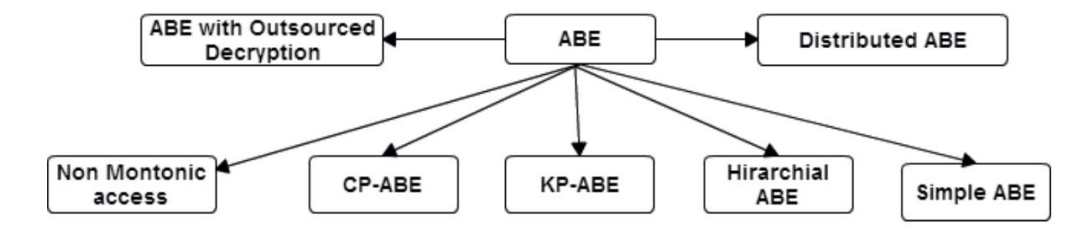
\includegraphics[scale=0.5]{graphics/chapter-2/chap2-abe-classified.png}
    \caption{Phân loại ABE \cite{kumar2015enhanced}}
    \label{fig:chap2-abe-classified}
\end{figure}
Trong phần tiếp theo, nhóm tác giả trình bày chi tiết thuật toán của hai phương
pháp mã hóa dựa trên thuộc tính trong Hình \ref{fig:chap2-abe-classified} là CP-ABE và KP-ABE. Đây là hai
phương pháp mã hóa nổi bật nhất. Các nghiên cứu về ABE theo hai hướng này ngày
càng rộng và tăng nhanh. \\
\indent Cả KP-ABE và CP-ABE đều sử dụng chung một cấu trúc truy cập, được gọi là
cây truy cập. Gọi $\tau $ là một cây biểu thị cấu trúc truy cập. Mỗi điểm nút trong cây là một cổng truy cập. Một cổng có cấu trúc bao gồm các nút con của nó và một giá trị cổng. Giả sử $\textbf{\textit{n}}_x$ là số lượng nút của của nút $\textbf{x}$ và $\textbf{\textit{t}}_x$ là giá trị cổng thì ta có $0 < \textit{t}_x \leq \textit{n}_x$. Nếu $\textit{t}_x = 1$ thì cổng đó là cổng $OR$, và ngược lại, nếu $\textit{t}_x = \textit{n}_x$ thì đó là cổng $AND$. Mỗi nút lá (là
nút không có nút nào là nút con của nó) diễn giải một thuộc tính và có giá trị cổng $\textit{t}_x = 1$. Hàm $\textbf{\textit{att(x)}}$ lúc này trả về thuộc tính liên kết với nút lá $\textit{x}$. Mỗi nút trong $\tau$ được đánh số thứ tự duy nhất. Hàm $\textbf{\textit{index(x)}}$ trả về thứ tự của nó, hàm $\textbf{\textit{parent(x)}}$ trả về nút cha của nó.\\
\indent Giả sử $\tau$ là cây tru cập với nút gốc tại $\textit{x}, \tau_x$ là cây con của $\tau$ có nút gốc tại $\textit{x}$. Tập thuộc tính $\lambda$ được gọi là thỏa mãn $\tau_x$ nếu $\tau_x(\lambda) = 1$. Việc tính toán $\tau_x(\lambda)$ được thực hiện như sau:
\begin{itemize}
    \item Nếu $\textit{x}$ là nút lá, $\tau_x(\lambda) = 1 \iff \textit{att(x)} \in \lambda$
\end{itemize}